\documentclass[11pt]{ieeeconf}
\usepackage{lipsum}
\usepackage{graphicx}
\usepackage{float}
\usepackage{lettrine}
\usepackage{caption}



\newcommand\blfootnote[1]{%
  \begingroup
  \renewcommand\thefootnote{}\footnote{#1}%
  \addtocounter{footnote}{-1}%
  \endgroup
}

\title{Bumper Car Sumo}
\author{Jaden Simon, Melvin Bosnjak, Daniel Humeniuk,
 \textit{Students}, \textit{University of Utah}}

\begin{document}
\begin{titlepage}
  \centering
  \
  \vfil
  \Large ECE 3992\\
  \Large Spring 2019\\  
  \Large Jaden Simon, Melvin Bosnjak, Daniel Humeniuk\\  
  \Large Bumper Car Sumo\\
  \Large http://bumpercarsumo.weebly.com/\\
  \Large Initial Proposal Document\\
  \vfil
\end{titlepage}


\maketitle
\begin{abstract}
Americans aren’t having fun anymore. The weight of capitalism is forcing families to work 60 hour weeks for low, soul-crushing pay. So not only do Americans lack the time for fun, they often lack the funds as well, leading to inefficient forms of entertainment. People with low life satisfaction tend to be unproductive in both their social life and their work life. An affordable form of entertainment would increase profits for businesses, and create an upward spiral of enjoyment, therefore, increasing productivity. In order to promote this, our group is designing an affordable, battle royale style, bumper car sumo game. This proposal will describe the motivation, design, and resources needed for this project.
\end{abstract}

\section{Introduction}
\lettrine{T}{he} cost and entertainment efficiency of our game will be the most important criteria for success. Costs should be low enough that most people can afford to play, while our game should yield high levels of fun per minute played. Because entertainment value is our primary goal, costs will only have a secondary role in our design process. Battle royale games have become a major hit in the entertainment world due to their competitive nature, as such our team decided to create a game where player-controlled robots attempt to push each other out of an arena. Last player remaining wins. To facilitate gameplay, our robots need to be easily pushed around by other robots. Games that drag on forever with little action are not fun. Controls should be easy to enhance playability, though not too easy as complexity adds to the fun. We need some way to detect game conditions, such as when a robot is out of bounds or when a player wins. This could be done with a human referee, but that would take away immersion of the game. Because some players may not have friends to play with, it is desirable to have some sort of AI to play against. Competitive games are much more enjoyable with worthy opponents.

Since cost is a contributing factor to our design, we will want to use existing technologies as much as possible. Robots can be constructed as a two-wheeled platform with wireless modules, similar to a segway. For extra entertainment, a spherical shell could encase the robot, reducing its traction on the play surface. A player’s phone can be used as a controller if a suitable app is developed. This negates the cost of constructing our own controllers at the slight cost of reduced playability. Computer vision libraries could allow us to track the location of each robot if painted differently. Exact positioning solves the problem of detecting game conditions, plus giving us plenty of information to use for a basic AI. 

Our goal, above all else, is that our game is fun. Playtesting will be a major component of our design process, rethinking aspects of the game if we decide it is not fun. Costs will be mitigated, but entertainment value will never be sacrificed for savings. Smiles and laughs from players is our primary measure of success.

\section{Design}

\subsection{Outline}

The project will require new software and hardware. To complete the project, we will need controllers, robots, trackers, and a main control mechanism. The controllers will be implemented as a web page that can be reached from many mediums. The robots will be created with two DC motors that are connected to WiFi or Bluetooth and powered by a battery.  A tracking system can be implemented with video tracking technology. The main controller for the game will need to communicate with the tracker and controllers. We may elect to run the controller from a laptop or a custom made device. With these four components, the game will be able to be made into a reality. 

\subsection{Hub}

The Hub will be a Raspberry Pi device that will have four primary functions: To capture the game state from a camera peripheral, use computer vision to keep track of each robots location, host a web server that will have bi-directional communication with the controllers, and wifi communication to relay the players commands to their respective robots. Fig. 1. shows the basic illustration of the game.

 \begin{figure*}[!t]
  \centering
  \captionsetup{justification=centering}
      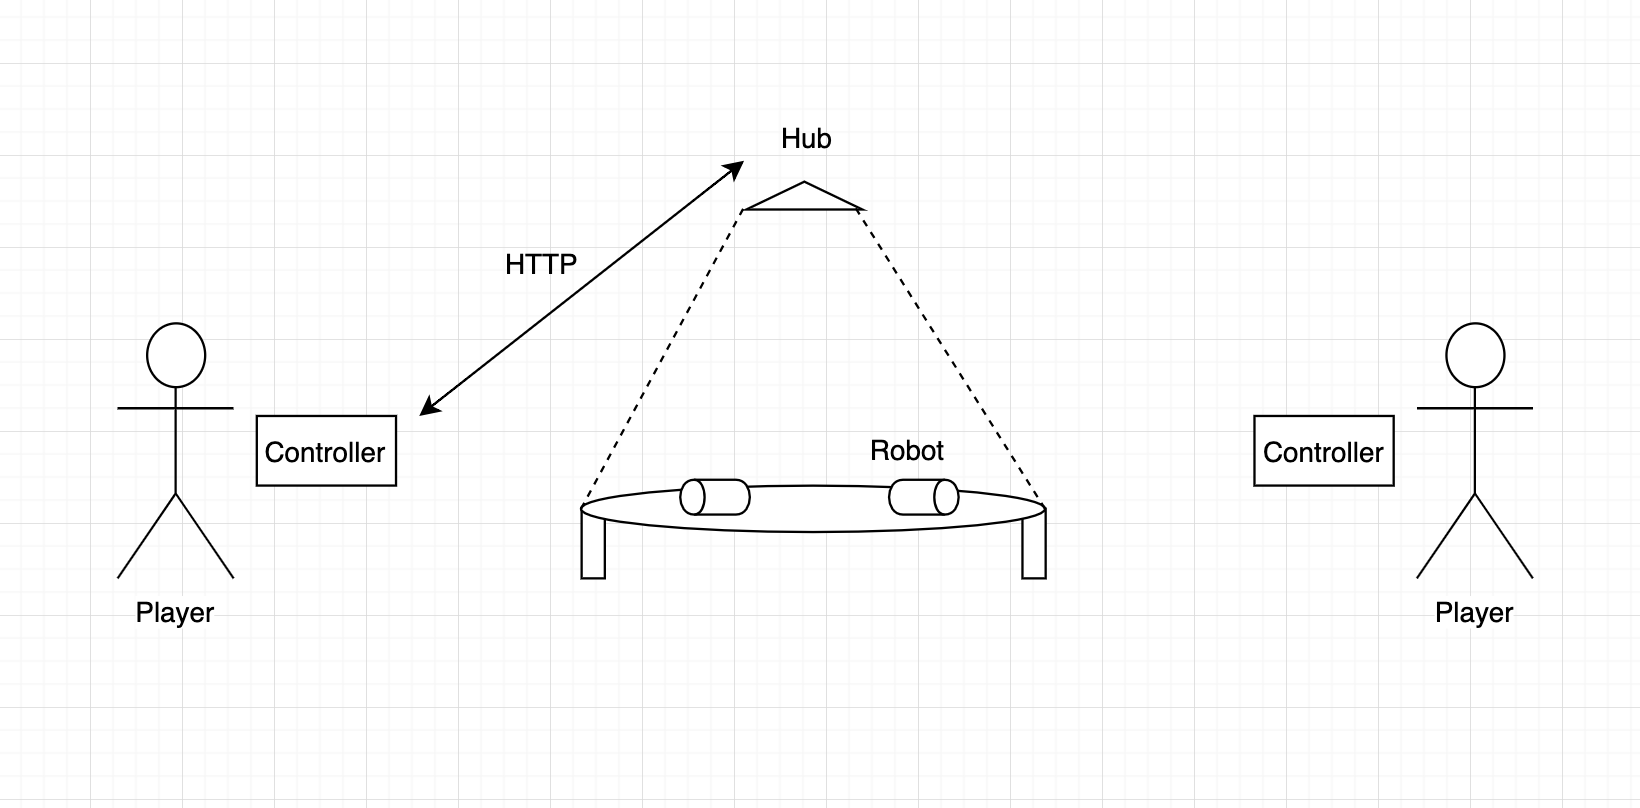
\includegraphics[width=14cm]{images/Overall.png}
        \caption{The design for the overall game.}
        \label{Illustration}
\end{figure*}

\subsection{Robot}

The robot will be a cylindrical shape with two wheels on each side of the body that can move in either direction. The robot will look similar to Fig. 2. In order to move forward, both of the wheels will spin at the same time at the same rate. To move backwards, the same principle applies in the opposite direction. To rotate the robot right or left the wheels will spin in opposite directions. In order to facilitate these functions in each robot, we will have two DC motors spinning the wheels. The DC motors will be controlled by a micro-controller that will be WiFi or bluetooth communication compatible. The micro-controller will get information from the main controller which will send it commands such as rotate right, rotate left, move forward, and move backward. The robot's micro-controller will then take this command and compile it down to its DC motor translation mentioned earlier.

 \begin{figure}[h]
  \centering
      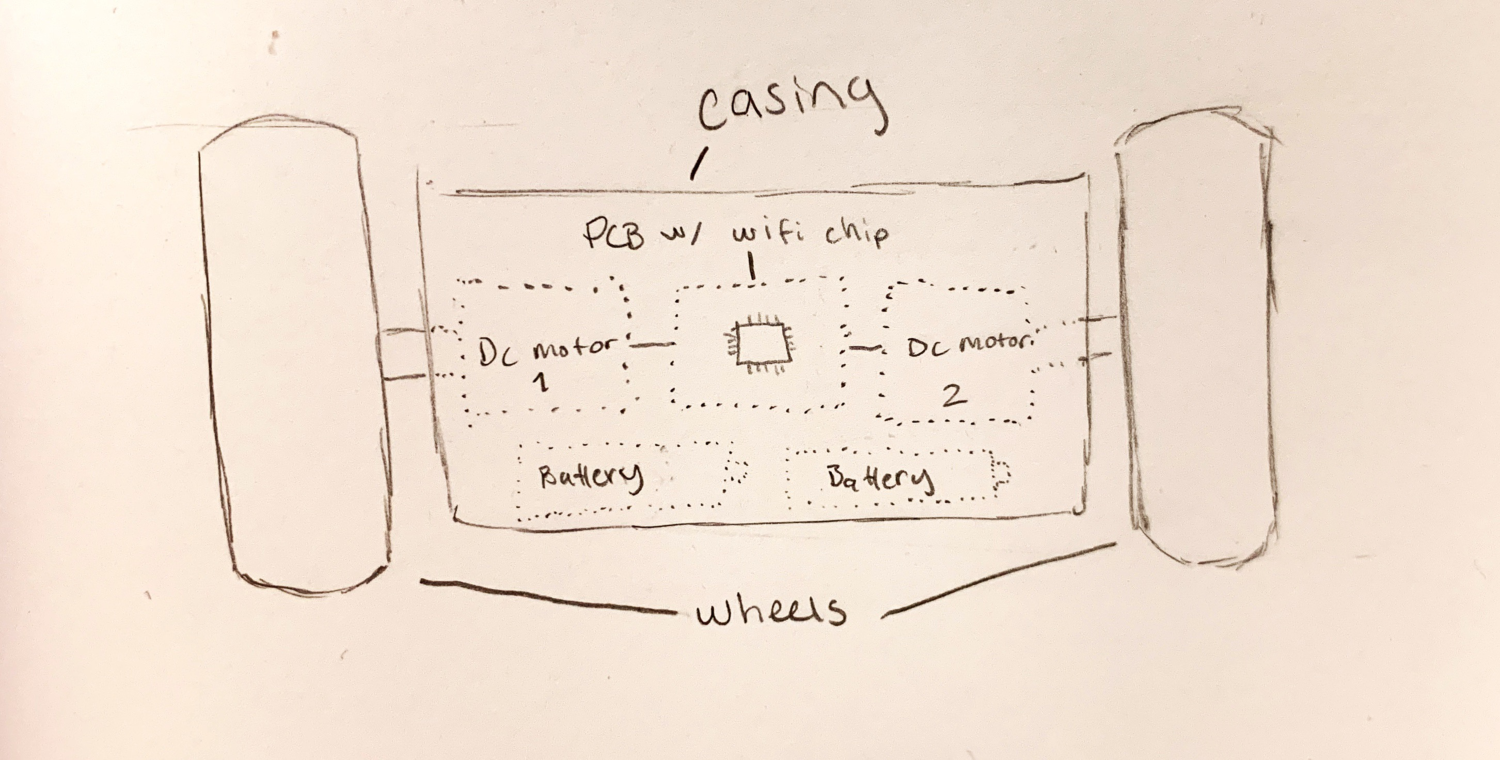
\includegraphics[width=0.5\textwidth]{images/RobotSketch.pdf}
        \caption{The design for the robot each player will control.}
        \label{RobotFig}
\end{figure}

\subsection{Controller}

The controllers will be any sort of device that can access the internet. Players will use their device to connect to the Hub by accessing a web page. This web page will be running a web server that is in constant communication with the robots. Once the player goes to the web page they will be prompted with available robots. If there is an available robot, the user will then choose and connect to that robot. Now that the player is mapped to that robot it will be constantly communicating its movement requests to the web server which will propagate it to the robot. The controller interface will be the arrow keys for a computer and buttons for a phone. The forward and backward movements will correspond to the up and down arrow keys, and the rotate right and rotate left movements will correspond to the right and left arrow keys. The web page will also send the player devices information about the game state such as players still active and possibly a live feed of the game.

\subsection{Tracking}

Tracking will be done by the Hub using a camera and an open source computer vision library called OpenCV that will process each frame from the camera. When we design the casing for each robot we will make sure to make them distinct colors so it will be easier to contrast each robot. The tracking is used in order to recognize when a player has been eliminated from the playing field so that we can update the game state and broadcast which players are still active to the controllers. It will also restrict any commands to robots that have been eliminated.

\section{Game Mechanics}

The style of this game can be described as battle royale mixed with bumper car sumo. In other words, bumper cars will be put on a platform and try to knock each other out of the play area. Last one standing wins. 

\subsection{Setup}

The hub will start up the server which will then wait for player connections to populate the game. Each player will navigate to the website and they will be prompted to choose an available robot. Once each robot is reserved, the hub will broadcast a countdown to each controller until the game starts. 

\subsection{Game Loop}

Once the countdown reaches zero the game will begin. Each controller will then be able to send commands to the hub which will propagate to the robot if it's still active. The goal for each player is to stay on the platform while trying to use its robots to physically push all other opponents off of the platform. The game will continue until all but one robot remain. Once only one robot remains, the hub will broadcast the winning robot to each controller and reset the game state into the Game setup. 

\section{Resources}

This project will demand a fair amount of resources. Each robot will require 2 DC motors, 2 350 mAh LiPo batteries, 2 wheels that the motors will rotate, PCB that includes an ESP8266 microcontroller and motor drivers for each DC motor, and a casing to enclose and protect the internals. The casing will likely have to be designed and 3D printed by our group.

The hub will require a Raspberry Pi to do the hub to controller communication, hub to robot communication, and the image capture and processing. The Raspberry Pi 3 Model B+ has a quad core 1.4GHz processor which should be enough processing power for these tasks. The hub will also require a camera peripheral that is compatible with the Raspberry Pi. The options for the camera are the Raspberry Pi camera, and the Logitech C922x Pro Stream Webcam. 

The playing field will be constructed out of a simple table top with some 2 x 4's to hoist up the camera.

Since the controller can be any device that has internet capabilities, there will not be a need for additional resources.

\section{Timeline}

\subsection{Spring}
For this semester, we will utilize our embedded systems final project to develop and test our wifi communication with the ESP8266 as well as motor control. This should be enough to prototype and demo some basic wireless robot control. 

\subsection{Summer}
The summer will consist of ordering and gathering the resources needed as well as detailed design for each component of the project. 

\subsection{Fall}
Most of the legwork for the project will be done during the fall. With all components gathered and the design completed all that will be left to do is to assemble and test. We will attempt to have everything assembled a month before demo to account for bugs and unforeseen problems.

% \nocite{*}
% \bibliographystyle{IEEEtran}
% \bibliography{IEEEabrv,bib/ref.bib}
\end{document}

% \begin{figure}[h]
%   \centering
%       \includegraphics[width=0.5\textwidth]{images/Figure1.jpg}
%         \caption{The two possible states Schrodinger’s cat could be observed as when the box is opened. \cite{Image}}
% \end{figure}